\documentclass{article}
\usepackage{graphicx}
\usepackage{xcolor}
\usepackage{subcaption}
\usepackage[margin=1.0in]{geometry}
\usepackage{float}
\usepackage{ulem}

\begin{document}
\section{Introduction}
\begin{enumerate}
\item \textbf{General goal}
Systematically develop model Hamiltonians which can accurately describe the energies and properties of the lowest lying eigenstates for strongly correlated electrons systems.

\item \textbf{Barrier to achieving that goal} The necessity for many-body interactions in describing the low-lying excited states of strongly correlated electron systems poses a difficult challenge when developing model Hamiltonians.

\item \textbf{State of the art} Common approaches to building these model Hamiltonians use effective single particle theories like density functional theory (DFT) to generate an effective 1-body model or build phenomenological models based on experimental measurements of the properties and energies of low-lying excitations.
\textcolor{red}{Have to find references for this one, not sure how true this is.}

\item\textbf{How are we advancing state of the art} In this paper we systematically fit a many-body model which can accurately describe energies and properties of low-lying eigenstates for the neutral CuO molecule using a generalizable \textit{ab-initio} Quantum Monte Carlo (QMC) density matrix downfolding (DMD) method, and discuss the details of and developments in the model fitting procedure.
\end{enumerate}

\section{Methods}
\begin{enumerate}
\item \textbf{Density matrix downfolding} The DMD procedure allows us to develop low-energy effective theories for physical systems in a systematic manner beginning with the \textit{ab-initio} Hamiltonian $H_{ab}$.

\item \textbf{Defining the low-energy space} We define the low-energy space for the CuO molecule as the full space of states with 9 to 10 electrons in the Cu 3d orbitals.

\item \textbf{Sample states} Our sample space (SS) was generated by sampling the span of base states - states which approximately describe true eigenstates within the LES - using multi-Slater-Jastrow trial wave functions in Diffusion Monte Carlo (DMC).

\item \textbf{Model basis} We constructed two bases for our model Hamiltonian, a localized intrinsic atomic orbital (IAO) basis for evaluating two-body reduced density matrix (2-rdm) elements, and a molecular orbital (MO) basis for one-body reduced density matrix (1-rdm) elements.

\item \textbf{Model selection and fitting}
\begin{enumerate}
\item We initially narrowed down the space of potential models by discarding any which did not at minimum contain descriptors essential in describing the low-energy space: $n_{4s}, n_{2p_\pi}, n_{2p_z}, \Sigma_{J_{sd}}, \Sigma_{U_s}$. \textcolor{red}{"Essential" should be determined through experimental knowledge + variation of descriptors within our SS}.

\item After fitting each potential model using ordinary linear regression (OLS) and solving the resultant models using exact diagonalization, we find a set of models which describe the energy functional on our SS accurately but whose eigenstates and spectra differ. \textcolor{red}{Need a figure to show this.}

\item Our inability to sample certain states within our target LE space manifests itself through intruder eigenstates within our fit models.

\item In order to ensure that intruder states are not present within our final model, we enforce a prior that pushes intruder states above a chosen $E_{cut}$ = 2eV by altering the cost function for our regression. 
\end{enumerate}
\end{enumerate}

\section{Discussion}
\begin{enumerate}
\item \textbf{Regression with prior} Using our new cost function we find a set of models which accurately describe the energy functional on our SS, have similar spectra and eigenvectors, and do not contain  intruder states below a cutoff energy $E_{cut} $= 2eV.

\item \textbf{Comparison to experiment} The selected low-energy model accurately describes the energies and single particle properties of the low-energy eigenstates of CuO as measured in experiment.

\item \textbf{Comparison to DFT} Our model is more accurate than a single-particle model constructed using density functional theory orbitals and eigenvalues.
\end{enumerate}

\section{Conclusion}
\begin{enumerate}
\item \textbf{Our findings} In this paper we systematically fit a many-body model for the neutral CuO molecule which can accurately reproduce the spectrum and properties of low-lying eigenstates seen in experiment using a \textit{ab-initio} Quantum Monte Carlo (QMC) density matrix downfolding (DMD) method, and discuss the details of and developments in our model fitting procedure.

\item \textbf{Avenues of interest} The fitting procedure illustrated here can be extended to other neutral transition metal oxide molecules, allowing for the construction of a sequence of low-energy models across the transition metals.
\end{enumerate}

\pagebreak
\section{Figures}
\begin{figure}[H]
\centering
\begin{subfigure}{.4\textwidth}
  \centering
  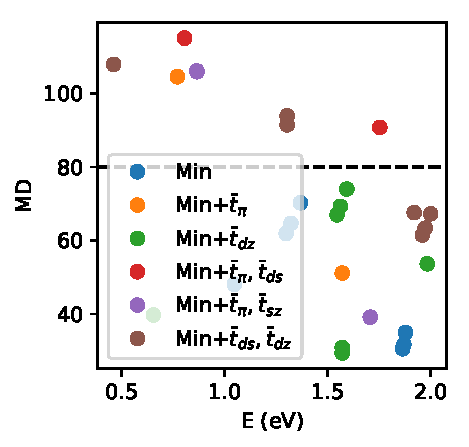
\includegraphics[width=\linewidth]{../qwalk/old/ub3lyp_s1_/analysis/figs/MD.pdf}
  \caption{Mahalanobis distances of excited eigenstates below 2eV.}
  \label{fig:Intruder1}
\end{subfigure}%
\begin{subfigure}{.5\textwidth}
  \centering
  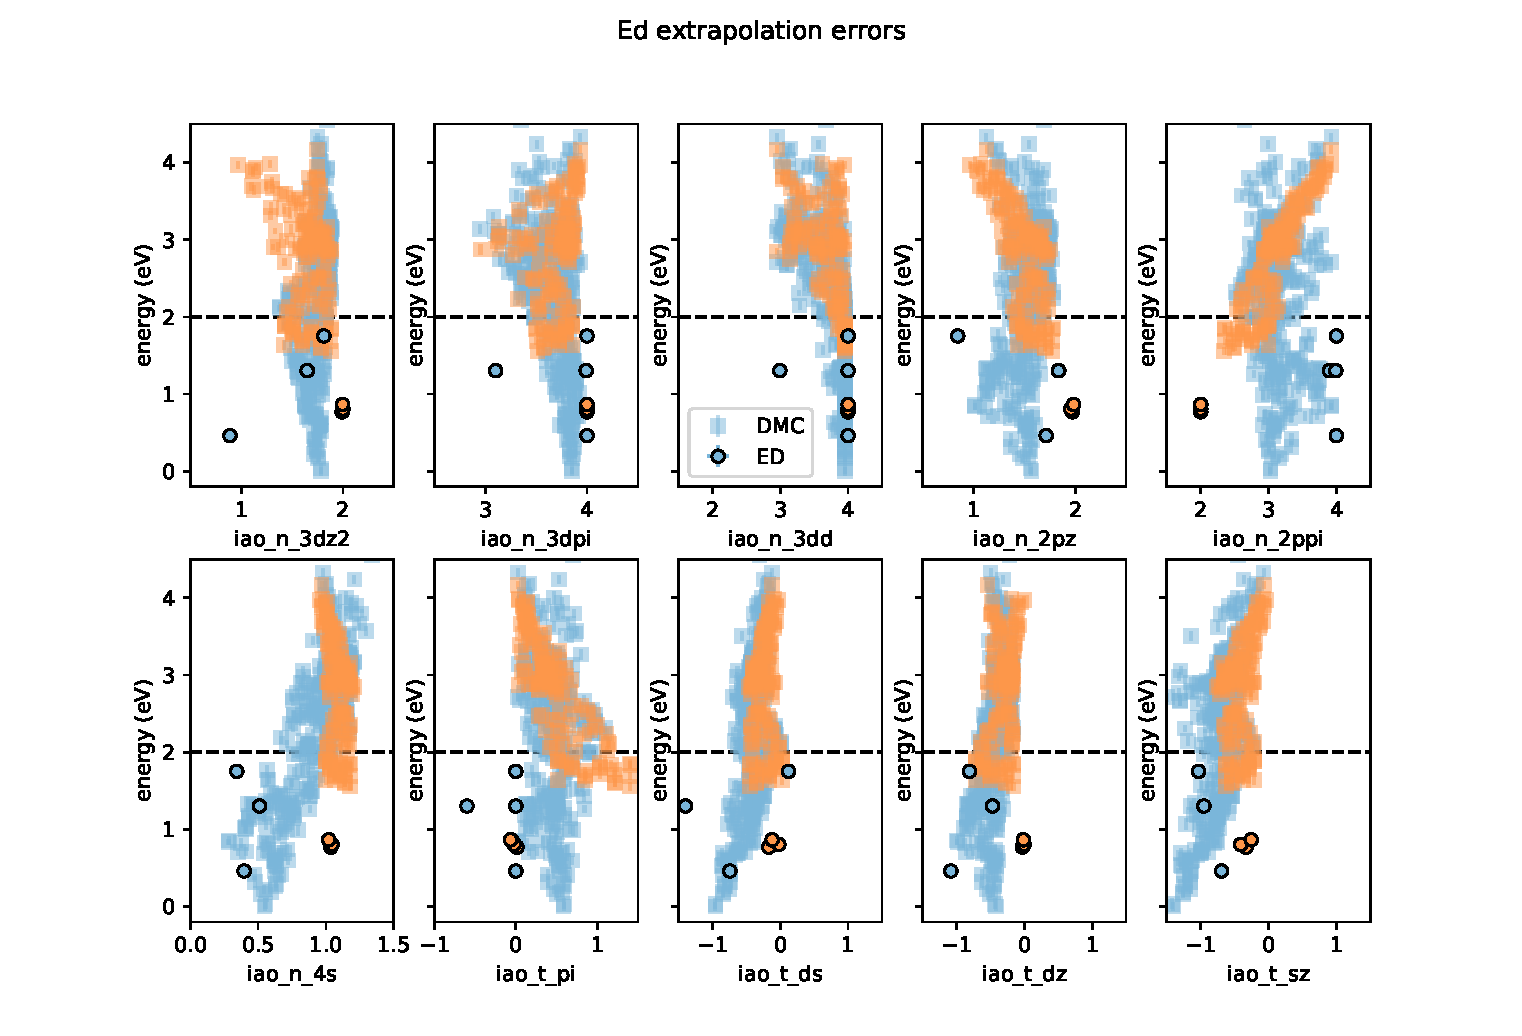
\includegraphics[width=\linewidth]{../qwalk/old/ub3lyp_s1_/analysis/figs/intruders.pdf}
  \caption{Properties and energies of intruder states.}
  \label{fig:Intruder2}
\end{subfigure}
\label{fig:Intruder}
\caption{a) The selection process for intruder states. Any excited eigenstates below 2eV with a Mahalanobis distance greater than 80 away from our SS are considered intruder states. b) The properties and energies of the selected intruder states.}
\end{figure}

\begin{figure}[H]
\centering
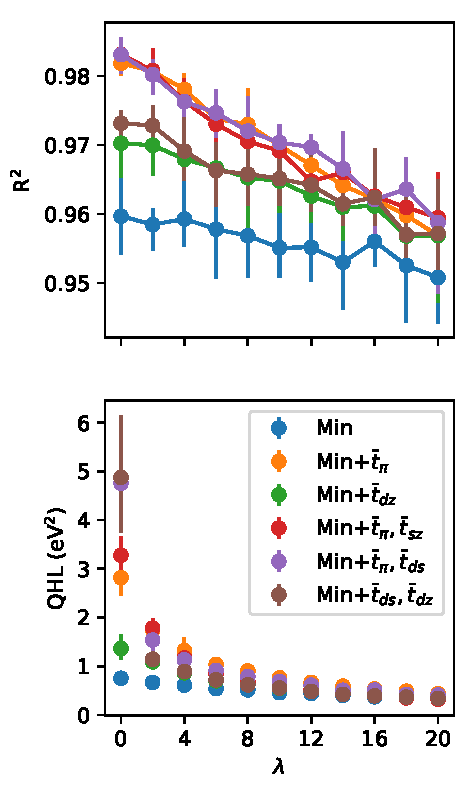
\includegraphics[width=0.7\linewidth]{../qwalk/old/ub3lyp_s1_/analysis/figs/prior.pdf}
\label{fig:Prior}
\caption{The $R^2$ scores and quadratic hinge loss versus $\lambda$ for the prior regression on the different models under consideration. The quadratic hinge loss converges to a single value for all six selected models as $\lambda$ is increased to 20 while the $R^2$ score stays above 0.95.}
\end{figure}

\begin{figure}[H]
\centering
\begin{subfigure}{.5\textwidth}
  \centering
  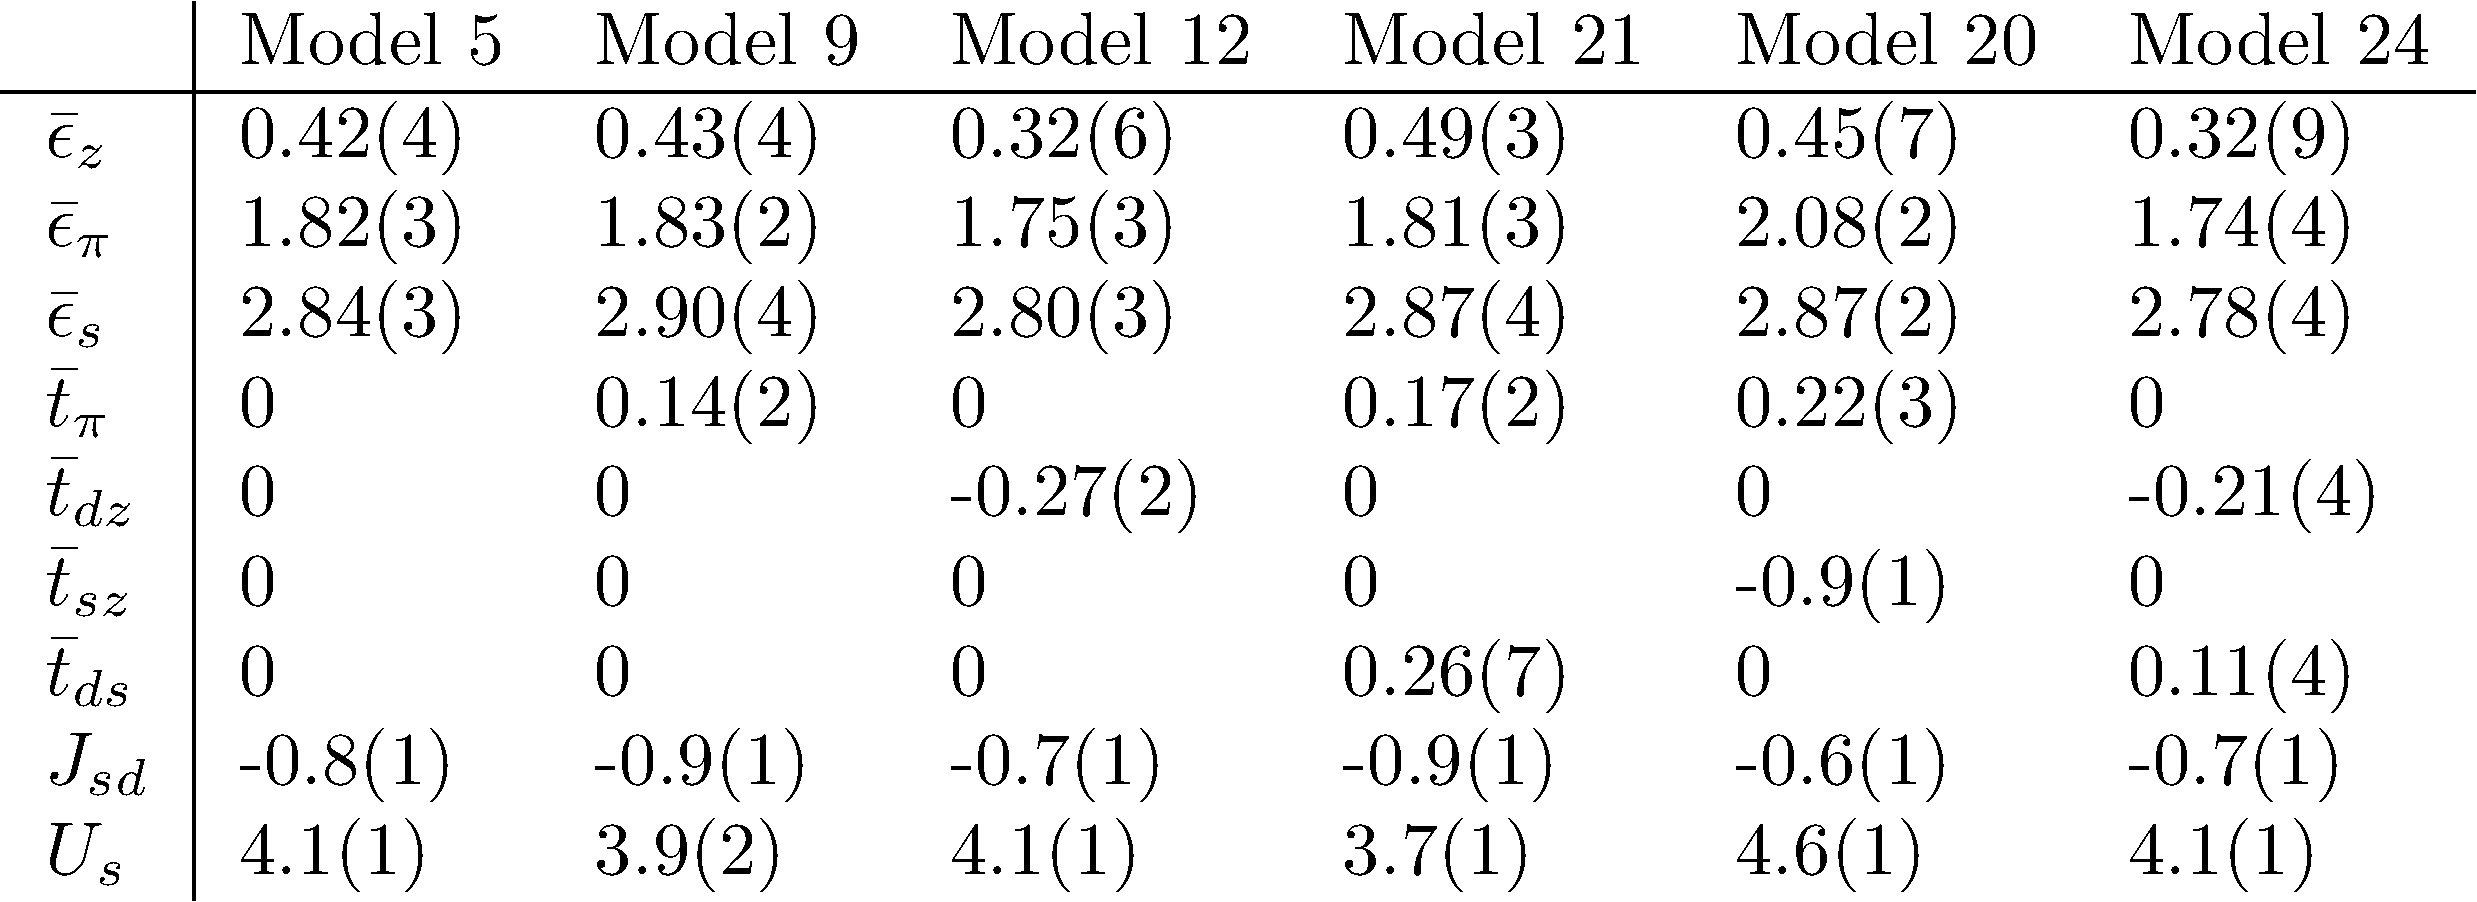
\includegraphics[width=\linewidth]{../qwalk/old/ub3lyp_s1_/analysis/figs/params.pdf}
  \label{fig:Params1}
\end{subfigure}%
\begin{subfigure}{.5\textwidth}
  \centering
  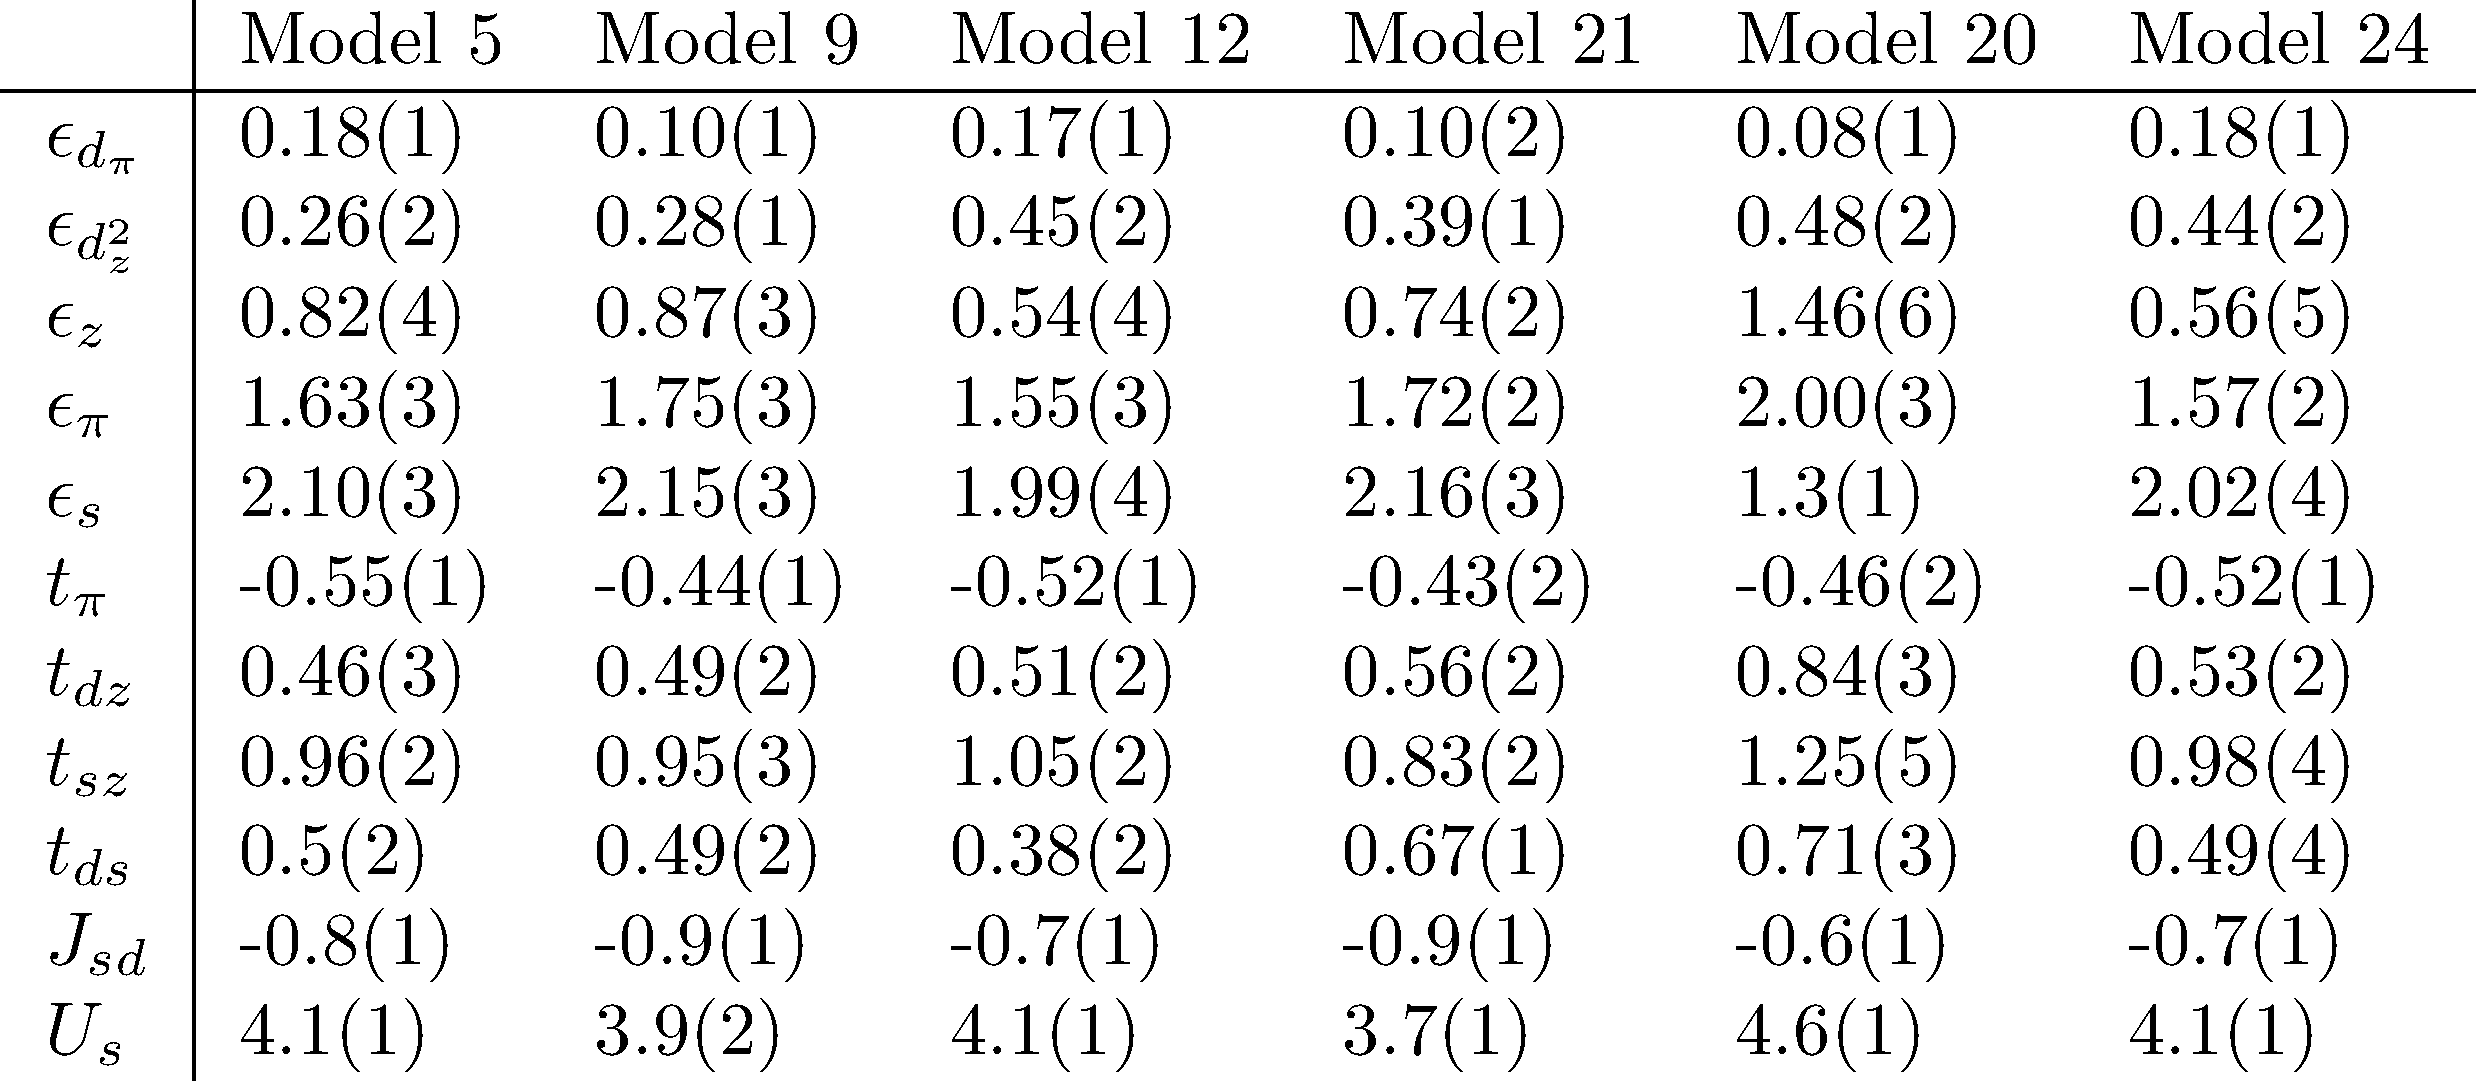
\includegraphics[width=\linewidth]{../qwalk/old/ub3lyp_s1_/analysis/figs/params_iao.pdf}
  \label{fig:Params2}
\end{subfigure}
\label{fig:Params}
\caption{The parameters fit for six different models using the prior cost function with $\lambda = 20$. On the left have the 1-body parameters in the MO basis and the right have the 1-body parameters in the IAO basis.}
\end{figure}

\begin{figure}[H]
\centering
\begin{subfigure}{.5\textwidth}
  \centering
  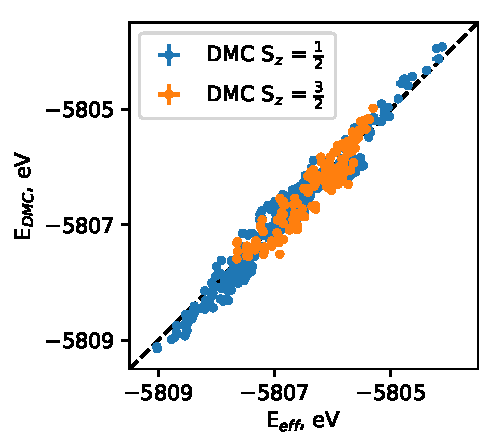
\includegraphics[width=\linewidth]{../qwalk/old/ub3lyp_s1_/analysis/figs/regr_m5_l20.pdf}
  \caption{Predicted versus sampled energies.}
  \label{fig:Fit1}
\end{subfigure}%
\begin{subfigure}{.5\textwidth}
  \centering
  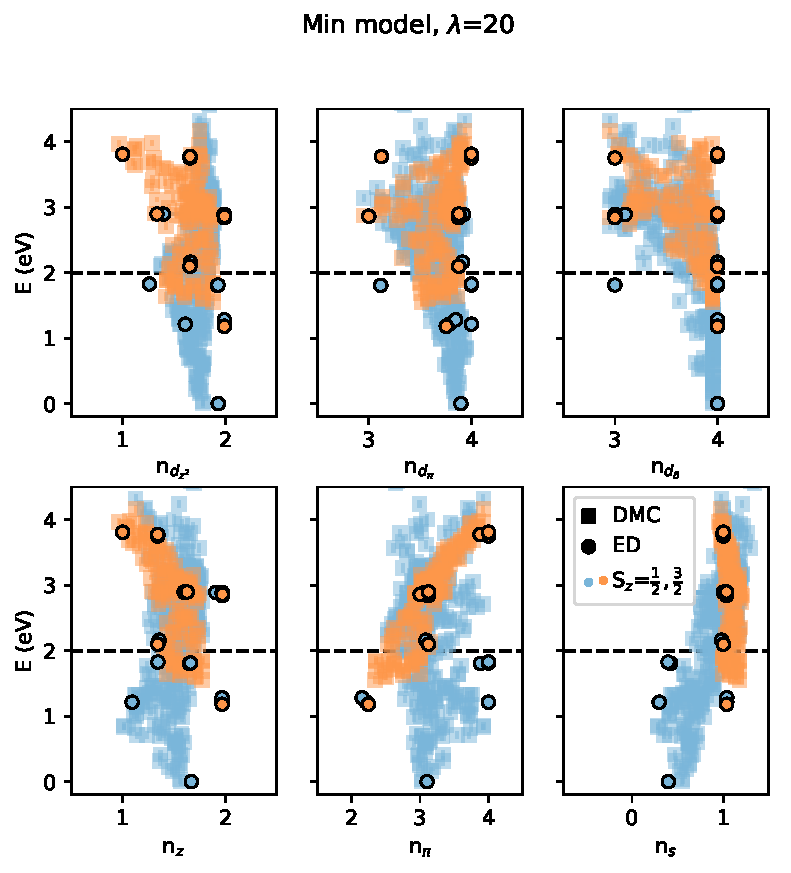
\includegraphics[width=\linewidth]{../qwalk/old/ub3lyp_s1_/analysis/figs/ed_m5_l20.pdf}
  \caption{Results of exact diagonalization.}
  \label{fig:Fit2}
\end{subfigure}
\label{fig:Fit}
\caption{The results of using the altered cost function with a prior to fit model 5 with $\lambda = 20$.}
\end{figure}
\end{document}